\subsection{Background}
\label{sec:background}

\subsubsection{Memory Translation Hardware}

\noindent
Modern computer systems use hardware-assisted memory translation,
	where the translation schemes are defined by the hardware architecture.
% The MMU performs the translation for each load and store instruction.
Upon a TLB miss, the MMU searches the translation structures (e.g., a page table)
%	and page walk caches)
	to obtain the translation---the virtual-to-physical address mapping.

\para{x86 Translation Scheme.}
%\label{sec:background:tree}
% Tree-based translation is the {\it de facto} scheme used by commodity systems.
All x86 processors since Intel 80386 have used a radix tree,
%	to record the mapping from virtual to physical addresses,
	as depicted in Figure~\ref{fig:background:radix-native}.
The depth of this tree has increased from two levels in 80386 to four levels in x86-64,
	with the fifth level upcoming~\cite{intel:5level,intel:5level:implement}
	and already supported in Linux~\cite{linux:5level-pt}.

\begin{figure}[H]
	\centering
%	\vspace{-15pt}
	\centering
	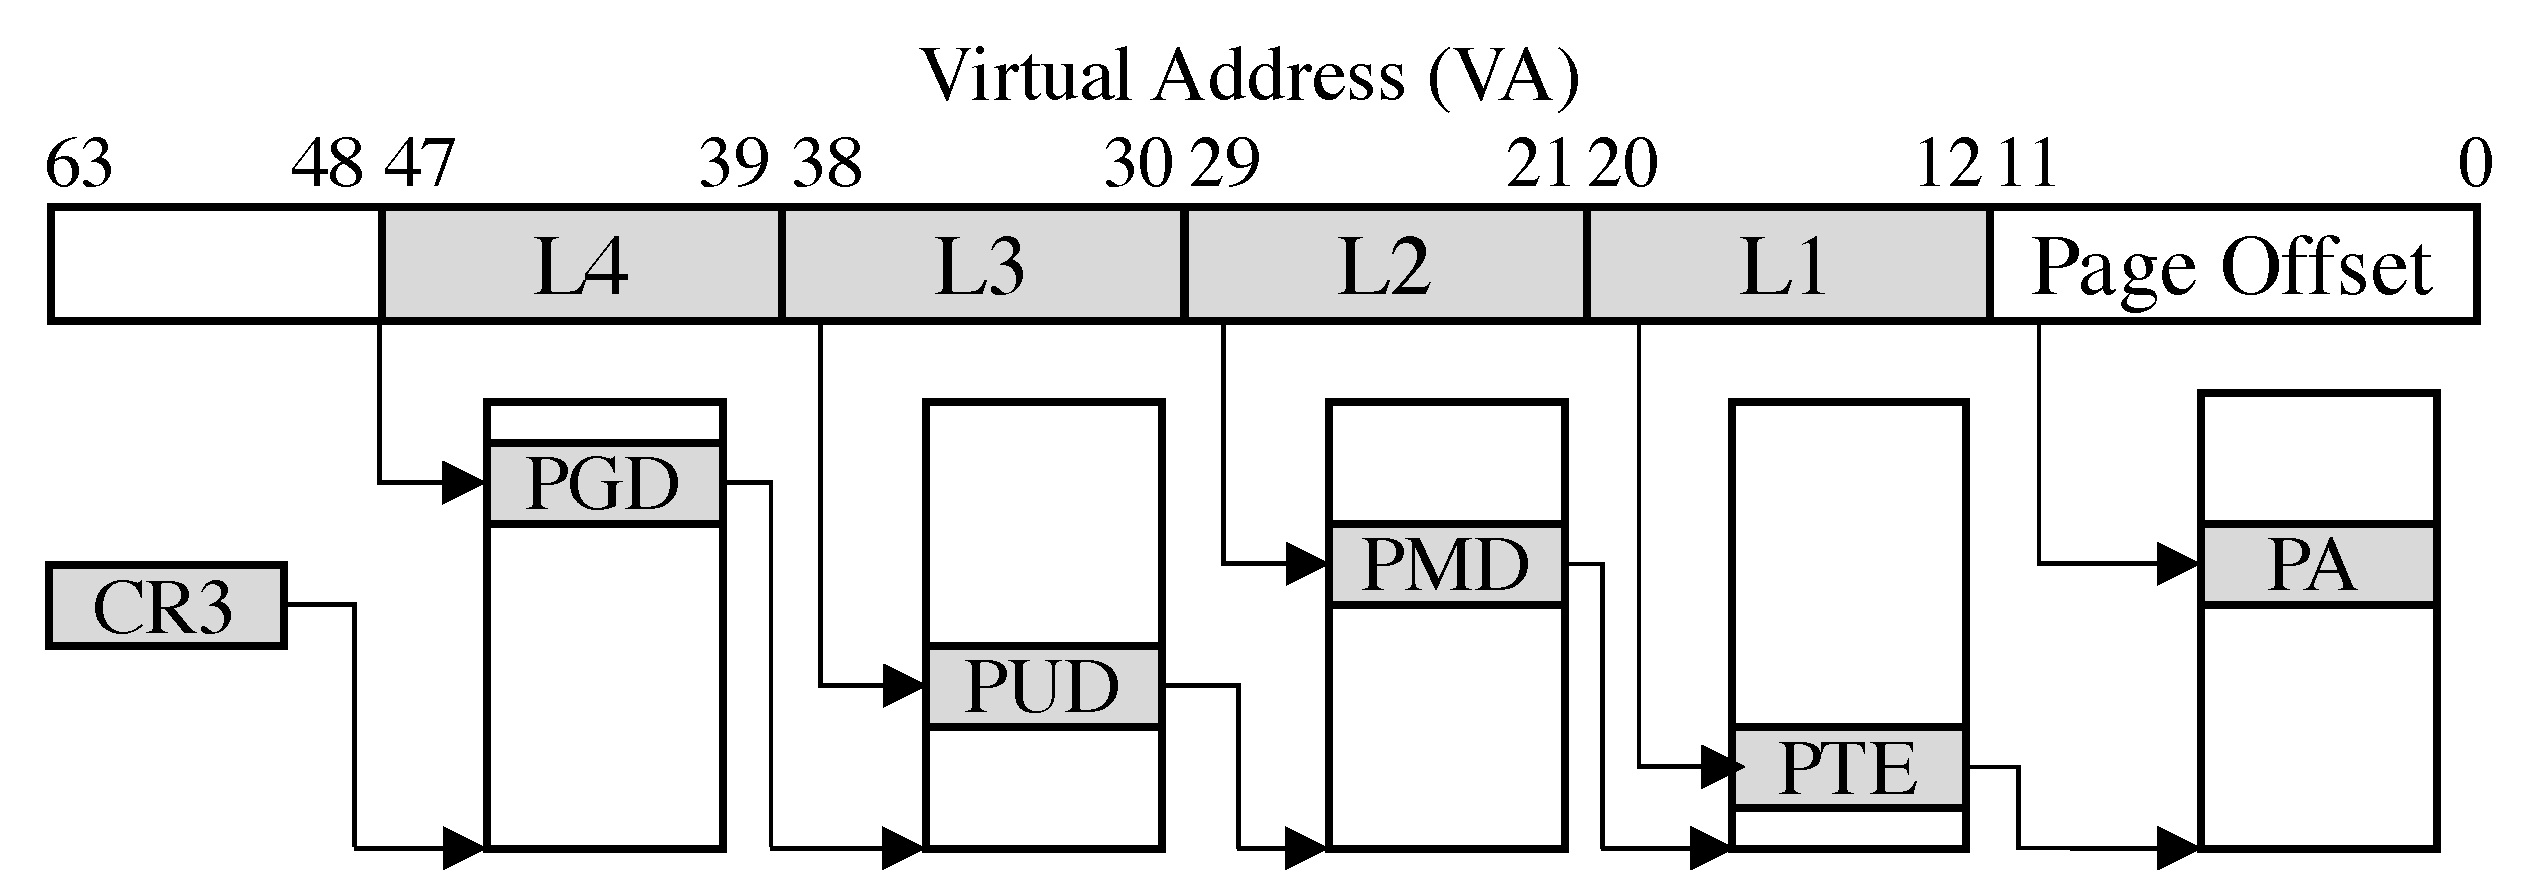
\includegraphics[width=0.475\textwidth]{figs/x86-walk}
	\caption{\bf Radix-tree based page table walk in x86-64 ISA.}
	\label{fig:background:radix-native}
\end{figure}

The main advantage of radix-tree based translation is space efficiency---tables at each level are created on demand---if at
	any level, no page is allocated within an address range, 
	the sub-tree is not allocated.
This yields significant memory savings, as the address space of 
	typical applications is sparse.

However, tree-based translation suffers from a major performance drawback---it 
	must {\it sequentially} walk the tree with multiple 
	memory accesses.
Page walk caches~\cite{barr2010translation,park2022fpt,bhattacharjee2013lmm} 
	and huge pages~\cite{navarro2002practical,kwon2016coordinated} are used to reduce the length of the walks,
	but struggle to address 
	emerging workloads with large memory footprints 
	and weak-locality access patterns.
The overhead %of tree-based translation 
	is further magnified 
	in {\it nested translation} for virtualized environments.
The MMU performs a two-dimensional walk over the guest and the host page tables.
%	where each access to the guest page table results in multiple accesses at the host.
A nested translation takes up to 24 sequential memory accesses with four-level page tables, 
	and up to 35 with five-level tables. 
It is reported that nested translation can take more than 50\% 
	of the execution time of memory-intensive workloads~\cite{alam2017doityourself,gandhi2016agile,margaritov2019asap}.
	% Recent studies~\cite{self:dmt} shows that, even everything is cached,
%	fetching 24 translation entries is a nontrivial overhead.
	
% It is reported that nested translation can take more than 50% of the execution time of memory-intensive workloads [6, 14, 23].

% \JZc{Here I use PSE for "translation entry from any level" and page directory for "page table pages".
% 1) PSE is from Intel manual, which they use for the same meaning. We use PTE in this paper as the Linux jargon for 4K pages. We may alternatively use "translation entry" if we want.
% 2) PD is the term that I invented. I don't want to use "page table page" here because AArch64 doesn't necessarily use a whole page}

% To translate a given virtual address (VA) into a physical address (PA),
%	the software or hardware must sequentially walk the tree,
%		and walk down recursively using the addresses and control bits stored in the related \ptes.
% Figure \ref{figure:background:radix-native} illustrates the process.

% Since multiple \ptes are referred to during the walk process, when creating and maintaining radix page tables,
%	the operating system may also need to check and update the status of other related \ptes.
% For example, to configure a PTE as writable, the system must set the PMD, PUD, and PGD to which it belongs as writable.
% However, to deny writes to a region of memory, it is only required that one of the parent \ptes is configured as unwritable.

\para{Flattened Page Table (FPT).}
Recently, extensive efforts are being made to optimize memory translation architectures.
A common principle is to shorten page table walks of the x86-64 scheme~\cite{park2022fpt,margaritov2019asap,
	ahn2012revisiting,karakostas2015redundant,alverti2020enhancing,gandhi2016agile,self:dmt}.
A recent proposal from Arm, known as Flattened Page Table or FPT~\cite{park2022fpt,Vougioukas2022fpt}, 
	flattens the x86 page tables by dynamically merging intermediate tree levels
	to reduce indirections and
	prioritize caching of page table entries.
Specifically, FPT tries to merge L4 and L3, as well as L2 and L1, in Figure~\ref{fig:background:radix-native},
	shortening the walk by half.

\para{Hashing-based Translation and ECPT.}
%\label{sec:background:ecpt}
Hashing is being actively revisited for translation~\cite{jovan2022nestedecpt,skarlatos2020ecpt,jovan2023memory,yaniv2016hash,vmware2021hashing,kanellopoulos2023utopia,gosakan2023mosaic, Kwon24}.
%To address the limitations of tree-based translation,
%	extensive efforts have been made to .
We focus on ECPT (Elastic Cuckoo Page Table)~\cite{skarlatos2020ecpt},
	a new hashing-based scheme
	which effectively speeds up translation with fully parallel lookups
	of page table entries.
%	reduce translation overhead by an average of 41\% over x86-64. %'s radix-tree scheme. % (\S\ref{sec:background:tree})
%	and is applicable to nested translation~\cite{jovan2022nestedecpt}.

% ECPT is an experimental architecture that is drastically different 
%	from x86-64, and thus help understand the extent of pragmatic OS framework,
%	compared with architectures designed with x86 compatibility (e.g.,~\cite{margaritov2019asap,self:dmt}).
% ECPT represents vast majority of new designs 
%	that attempt to preserve existing virtual memory abstractions, instead of 
%	removing them~\cite{}. 
	
%	or rebooting them~\cite{gupta2021midgard}
%	(which argubly would benefit more from a clean-slate OS than 
%	improving extensibility of existing ones).

Figure~\ref{fig:background:ecpt-native} depicts ECPT-based memory translation.
% In a nutshell, ECPT is an advanced hashing-based translation architecture. 
Different from conventional hashed 
	page tables~\cite{yaniv2016hash,Dougan:1999,huck1993architectural,talluri1995pagetable,Gray05}, 
	ECPT uses process-private hashed page tables that are dynamically resized based on occupancy.
ECPT uses Cuckoo Hashing~\cite{pagh2004cuckoo} and maintains multiple tables (called {\it ways})
	to proactively resolve hash collisions 
	by moving entries across ways.
% \schaix{The ways can be looked up 
% 	in parallel by MMUs to harvest memory parallelism and eliminate sequential tree walks
% 	ECPT maintains multiple page tables, corresponding to 
% 	different page sizes (e.g., 1GB, 2MB, and 4KB pages).}
\schai{During a page table walks, the MMU computes hashes of the Virtual Page Number (VPN) 
	to look up the ways in parallel.
It eliminates the need for sequential tree walks.
ECPT supports multiple page sizes (e.g., 1GB, 2MB, and 4KB pages) 
by maintaining a set of hash page tables for each page size.}

%, which issues six parallel lookups 
%	to six ways of three page tables (for 1GB, 2MB, and 4KB pages).

To reduce parallel lookups, 
	ECPT uses an in-memory data structure named Cuckoo Walk Table (CWT);
	each CWT
	maintains metadata (size and way) of ECPT translation entries.  
	% of recently accessed pages of each page table.
CWTs are cached in special MMU caches named Cuckoo Walk Caches (CWCs).
During translation, if a requested page hits a CWC, the MMU can directly look up the specific
	page table (with the size) or the specific way.
% state-of-the-art novel address translation design that
%	uses read-optimized cuckoo hash tables to replace radix-trees.
% It is designed to reduce the expensive address translation overhead that stems from sequential page walks.

% ECPT uses several physically-contiguous hash tables to store \ptes.
% In an ECPT, the hash tables are organized into \textit{ways}, with each way recording the \ptes that maps pages of a particular granularity.
% The ways are subsequently used for address translation of pages at different granularities.
% Note that, due to hashing, physically adjacent \ptes may map discrete virtual memory regions.\JZc{TODO: Seems we need to settle the meaning of term "way"}

% Figure \ref{figure:background:ecpt-native} illustrates the page walk of ECPT.
% When translating a VA, the page table walker calculates the hashes for the VA, accesses all ways that the \pte \textit{may} present in parallel,
%	and fetches all entries at the calculated hash table slots.
% The walker then checks the tags of each obtained entries and consumes the one with the right VA for translation.


% ECPT only tracks \ptes that directly maps a page, hence the OS must ensure that each VA and its \pte are only recorded by at most one hash table
%	to avoid ambiguity in the translation process.
% To avoid hash collisions, the OS may increase the size of the hash table when it exceeds a predetermined threshold or when a collision occurs.
% This process is called \textit{rehashing}.
% To reduce memory bandwidth usage, ECPT employs 
%	to help the walker decide which ways it should send requests to.

% \para{Other translation designs.}
% In recent years, several other novel address translation designs have been proposed.
% Direct Memory Translation uses physically contiguous Translation Entry Areas to provide single-access translation capability for radix page tables.
% Flattened Page Table uses a larger page directory size to reduce the number of levels in a radix page table.
% Hashed Page Table uses an open-addressing hash table instead of a radix page table.
% Mosaic Page compresses \ptes by bucketing physical memory to improve cache hit rates.

% All of the above novel designs exhibit good address translation performance in hardware simulation.
% However, due to the lack of system software support, the software implications of these designs have yet to be fully understood.

\begin{figure}[H]
	\centering
	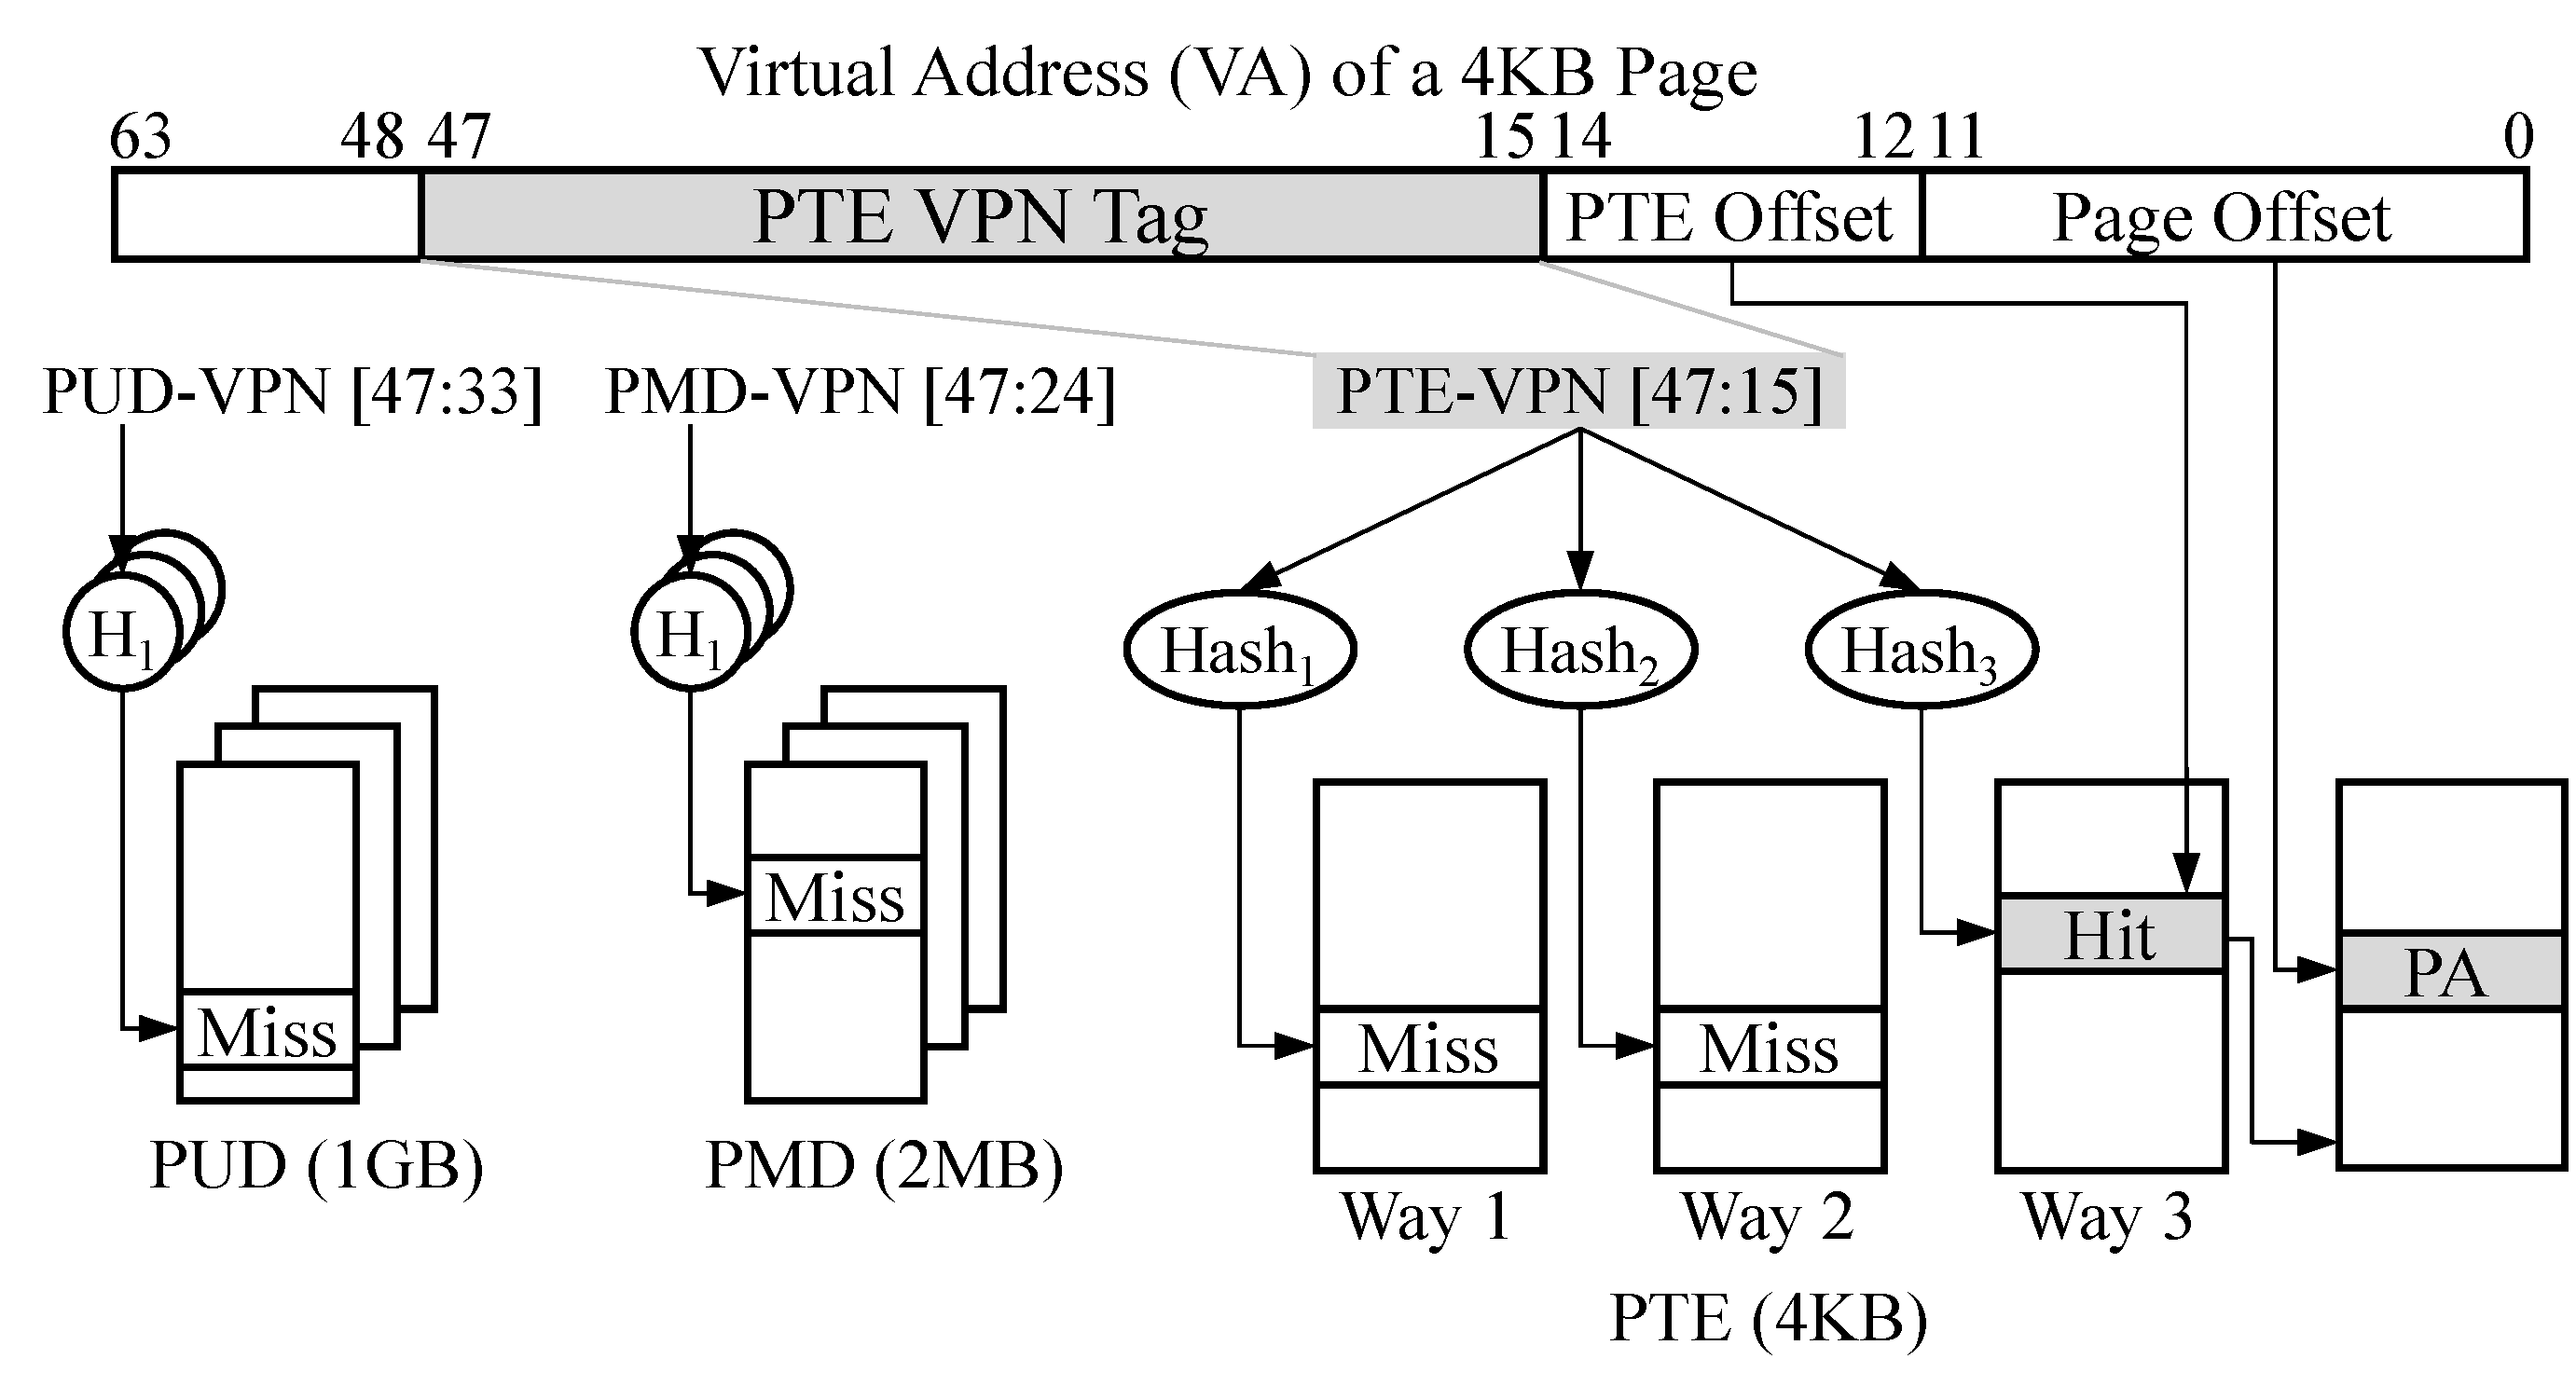
\includegraphics[width=0.475\textwidth]{figs/cuckoo-walk-v3}
	\caption{\bf Parallel page-table lookup in an ECPT-based architecture~\cite{skarlatos2020ecpt}
		using three-way cuckoo hashing.}
	\label{fig:background:ecpt-native}
\end{figure}

\subsubsection{OS Memory Management}
\label{sec:background:mm}

\noindent
The OS manages in-memory translation structures like page tables
	and other auxiliary structures (e.g., CWT in ECPT), defined by the hardware architecture.
%	for both user processes and the kernel itself.
The OS is also responsible for managing translation data
	(virtual-to-physical address mappings and metadata like protection and dirty bits).

Translation information is consumed by almost all OS memory 
	management operations.
% such as page-fault handling,
%	huge page management, page migration, etc.
Hence, translation architectures have strong implications on OS performance.
For example, recent work~\cite{yan2019nimble} shows that 
	the majority of page migration cost is from 
	OS memory management on translation-related operations 
	like unmapping/remapping pages and demoting huge pages,
	instead of actual page copies.
% \jzmark{Shall we say "a notable part of page migration cost" to be safe?}
% \TODO{@Jiyuan, @Siyuan, give an example, perhaps using our own evaluation
%	on page-fault handling,
%	that operations are important
%	in terms of performance? I think THP is one, but it's better 
%	to come from ours.}

Modern OSes separate {\it architecture-independent} OS memory management
	and {\it architecture-dependent} hardware support. % (e.g., code in ``\texttt{\small linux/mm}'' versus ``\texttt{\small linux/arch/x86/mm}'' in Linux).
Mach~\cite{accetta1986mach} designed a machine-independent memory manager where 
	its architecture-independent code 
	makes few assumptions about MMUs~\cite{rashid1987machine};
% All architecture-dependent code is encapsulated in a pmap module
%	which represents a general address map (e.g., a VAX page table~\cite{levy82virtual} and segment registers in IBM RT PC).
the design is inherited by BSD kernels~\cite{cranor99uvm}.
EMT is inspired by Mach/BSD, but focuses
	on empowering new, experimental translation schemes.
%	and enabling memory management to benefit from architecture-specific optimizations.

%	it exposes low-level primitives to OS memory management %like pointers to translation entries
%	and enables hardware-specific customizations on architecture-neutral implemenations. % on primitives iterators and locks.

Linux layers machine-independent/dependent code differently.
It maintains a multi-level tree-based page table in the architecture-independent module.
%	(architectures not using tree-based translation are expected to emulate the tree-based page table).
This design achieves high-performance memory management:
	1) it enables optimizations that need to directly 
	manipulate page tables and translation entries, % which is hard realize via pmap in BSD/Mach,
	and 2) it avoids overhead due to indirections.
However, it lacks extensibility to different translation architectures especially those
	that do not fit its tree definition such as ECPT or even the conventional hashed page tables.\footnote{
	% \footnote{\schaix{Hashed page tables (HPTs)
	% was provided by architectures like IA-64 and Power~\cite{ia64:man,ppc64:man};
	% Linux does not have native support for HPTs~\cite{linux:torvalds_pt}.}}
\schai{Hashed Page Tables (HPTs) was provided by architectures like IA-64 and POWER~\cite{ia64:man,ppc64:man},
	but Linux does not have native support for HPTs~\cite{linux:torvalds_pt}.
	Linux maintains a software tree-based page table to store full virtual memory mapping and treats the HPTs as soft-managed extended TLBs.
	Such an approach leads to duplication of translation data and redundant maintenance.}}

% even if the underlying architecture may not support it.

% To carry out memory management operations in a portable manner,
%	modern cross-architecture operating systems, such as Linux, FreeBSD, and ReactOS,
%	typically divides memory management into architecture-independent and architecture-dependent parts,
%		which are connected through an OS-specified translation interface.
% The architecture-independent part implements memory management logic such as memory allocation, fault handling, page migration, swapping, etc.
% The architecture-dependent part is responsible for translating the memory management demands
%	into concrete architectural operations.

% As the bridge between the two parts, the translation interface is the "language" used throughout the memory management subsystem.
% It not only transcribes the system's instructions to the architecture supports,
%	but may also determine whether certain operations are possible or not in the system
%		- because the architecture-dependent parts get much of the knowledge through instructions expressed in that interface.
% Hence, the interface has a critical impact on the scalability, performance, and maintainability of memory management.

% For example, compared to FreeBSD's Mach model, Linux's five-level page table model sacrifices extensibility,
%	but it exposes more optimization opportunities that are not possible in FreeBSD since the latter closely resembles what hardware sees.

% \para{Memory subsystem in Linux}
% \TODO{This paragraph is not correctly written.
% 	We need to start from the memory management subsystem
% 	before going directly to the page table---remember the figure we put in the Intel ArchFest slides?
% Seriously, the key points to make is (1) most of the mm kernel code is tightly 
% 	coupled with translation-related operations (how many are green 
% 	and how many are red -- we can bring the figure here),
% 	and (2) the current translation assumes a tree-based translation
% 	and is hard to change (no interface).
% The last sentence should transit naturally to the next section.}
% Following the aforementioned pattern, Linux's memory subsystem also consists of two parts.
% The architecture-independent part of Linux is responsible for a variety of functions including
% 	fault handling, huge page, NUMA policy, and memory hot plug.
% Through its five-level page table interface tailored to popular architectures,
%	all of these \textit{architecture-independent} functions directly manipulate the \textit{architecture-specific} page tables with near-zero overhead, enabling high-performance memory management.


% Such tight coupling also limits extensibility.
% Our communications with multiple vendors reveal that it is a popular belief that Linux's memory management lacks extensibility,
%	creating an enormous challenge for the rollout of new hardware designs.
% Due to its abstraction of a five-level page table,
%	it is difficult to retrofit non-radix tree designs such as ECPT for Linux's memory management.

% As such problems are becoming pronounced today due to the increasing demand for reducing translation overhead,
%	the need of a new translation interface that combines both performance and extensibility is again a topic that is worth discussing.

% The Linux kernel defines its page table abstraction as a hierarchy that is five levels in height, % https://docs.kernel.org/mm/page_tables.html
% 	closely resembling a five-level radix page table.
% The number of levels was deliberately chosen to support the five-level radix page table feature of x86-64. % https://lwn.net/Articles/717293/
% The page table abstraction is exclusively and universally adopted in the kernel
% 	and it is a documented requirement that all "architecture-neutral" codes must implement this abstraction. % https://docs.kernel.org/mm/page_tables.html

% Though this abstraction naturally fits popular hardware designs,
% 	it suffers from several known problems.
% The major problem of this abstraction is that it requires the developers of each architecture support to
% 	retrofit or disregard architectural features even though the abstraction should, in theory, be architecture-independent.
% In addition to this, although not declared, Linux widely defaults that virtually adjacent pages should have physically adjacent \ptes.
% It also assumes that any high-level \ptes is divisible and naturally encapsulates a set of lower-level \ptes at the virtual address.

% In practice, the current abstraction model already poses a challenge to the implementations of some architecture supports.
% For example, to support the four-level page tables currently commonly used by x86-64,
% 	the developers of x86-64 support codes must "fold" two levels of the five-level page table model so that they have the same semantics and behavior.
% However, the abstraction is still maintained in architecture-independent codes despite that the kernel community acknowledges some architectures do not support it. % https://docs.kernel.org/mm/page_tables.html, https://www.kernel.org/doc/gorman/html/understand/understand006.html

% (no!!!) don't add more load to reviewers!
% Linux uses % https://docs.kernel.org/mm/page_tables.html
%	PGD (Page Global Directory),
%	P4D (Page Level 4 Directory),
%	PUD (Page Upper Directory),
%	PMD (Page Middle Directory),
%	and PTE (Page Table Entry)
%		to refer to each of the five levels of the page table from top to bottom.
% In this paper, we will use the same terminology.
